% ============================================================================
%  Multi-Model Support for Blockchain-Based Business Processes
%  Extending Chorpiler for BPMN Process and Collaboration Diagrams
%  Tom Linus Köhler — Technical University of Munich
%
%  LNCS template.  You need Springer's `llncs.cls` and `splncs04.bst`
%  (available in the Overleaf "Springer LNCS" template, or from Springer).
%  Target length: ~10 pages.
%
% ============================================================================
\documentclass[runningheads]{llncs}

\usepackage{graphicx}
\usepackage{booktabs}
\usepackage{listings}
\usepackage{xcolor}
\usepackage{amsmath}
\usepackage[hidelinks]{hyperref}

% Solidity-ish listing style
\lstdefinestyle{sol}{
  basicstyle=\ttfamily\footnotesize,
  keywordstyle=\color{blue!60!black},
  commentstyle=\color{green!40!black},
  numbers=left, numberstyle=\tiny\color{gray},
  breaklines=true, frame=single, captionpos=b,
}
\lstset{style=sol}

\begin{document}

\title{Multi-Model Support for Blockchain-Based Business Processes: Extending Chorpiler for BPMN Process and Collaboration Diagrams}
\titlerunning{Multi-Model Support for Chorpiler}

\author{Tom Linus Köhler}
\authorrunning{T. L. Köhler}
\institute{Technical University of Munich \\ \email{tomlinus.koehler@tum.de}}

\maketitle

\begin{abstract}
Chorpiler compiles BPMN choreographies into gas-optimised Solidity smart contracts, but it does not support the two other BPMN model types, process and collaboration diagrams. This paper extends Chorpiler to both. The key observation is that all three diagram types map onto the same Interaction Petri Net, so the new support was added by extending only the parser. A process is treated as a choreography with a single default participant, and a collaboration as several processes composed in parallel and joined by merged message exchanges. We reuse the existing encoder, backend, and test harness, and contribute conforming and non-conforming test cases that validate the new diagram types on a local blockchain. We also compare the three diagram types and study how access control should be expressed for process diagrams, implementing three participant models. Measurements show that enforcing access control costs about 2{,}000 gas per task, and that deriving roles from lanes is no more expensive per task than using a single actor.
\keywords{Blockchain \and BPMN \and Smart Contracts \and Business Process
Execution \and Petri Nets \and Chorpiler.}
\end{abstract}

% ============================================================================
\section{Introduction}

\subsection{Context and Motivation}
Business processes increasingly span several organisations that must cooperate without fully trusting one another. In such settings a neutral party is normally needed to coordinate the process and to record what each participant has done. Blockchain technology offers an alternative to that trusted intermediary. A smart contract, that is, a program deployed on a blockchain, executes deterministically and is enforced by the network rather than by any single party, and its execution is recorded immutably. Encoding a business process as a smart contract therefore lets mutually distrusting organisations run the process with a shared guarantee on the order of steps and on who performed them. Compiling a process model directly into such a contract has been shown to be both feasible and efficient~\cite{garcia,weber}. 

\subsection{Problem Statement}
Chorpiler is a compiler that turns BPMN models into gas-optimised Solidity smart contracts~\cite{chorpiler}. In its current form it supports only one of the three BPMN model types, the choreography diagram. BPMN is also widely used through process diagrams, which describe the internal flow of a single organisation, and collaboration diagrams, which describe several organisations communicating through messages. A modeller who describes a process with either of these two notations cannot currently target Chorpiler, even though the underlying execution model is the same. This restricts the range of processes that can be compiled and excludes the diagram types that many modellers use most often.

\subsection{Objectives and Scope}
The goal of this work is to remove that restriction. Following the assigned task, it extends Chorpiler to support process and collaboration diagrams, provides an automated test suite for the new diagram types, and compares the features of all three BPMN model types. Beyond this scope, it also investigates how access control should be expressed for process diagrams, which natively have no participants, and implements and measures three alternative participant models. The main contributions are therefore the two new front-end translations, the automated tests that validate them on-chain, the feature comparison, and a quantitative comparison of the three access-control strategies.

\subsection{Structure of the Paper}
The remainder of this paper is structured as follows.
Section~\ref{sec:background} introduces the background on blockchain-based process execution, the Chorpiler framework, and BPMN.
Section~\ref{sec:comparison} compares the three BPMN diagram types. Section~\ref{sec:implementation} describes the design and implementation of the new support. Section~\ref{sec:testing}
presents the automated test suite and the evaluation results.
Section~\ref{sec:discussion} discusses the outcomes and limitations.

% ============================================================================
\section{Background and Foundations}
\label{sec:background}

\subsection{Blockchain-Based Business Processes}
A blockchain is a replicated, append-only ledger maintained by a network of nodes with no central authority. Modern blockchains such as Ethereum also run \emph{smart contracts}, which are programs stored on the ledger and executed by every node through a virtual machine. Because all nodes re-execute a contract and agree on the result, its behaviour is deterministic and cannot be altered by any single participant. Every state-changing call is a transaction sent from an account, and its computation is paid for in \emph{gas}, a unit that prices each operation. Reading and writing contract storage are among the most expensive operations, so the amount of storage a contract touches dominates its running cost. This property motivates compact state encodings and makes gas a meaningful measure when comparing contract variants. Running business processes on a blockchain in this way lets organisations that do not trust each other share a tamper-proof record of the process and a guarantee that its rules are followed~\cite{garcia}.

\subsection{The Chorpiler Framework}
Chorpiler is a compiler from BPMN models to Solidity smart contracts. It works in three stages. First, it parses a BPMN model into an Interaction Petri Net, a Petri net in which transitions represent interactions between participants~\cite{decker}. Second, it encodes this net as a compact state machine whose marking is stored in a single integer, where each bit corresponds to one place; this encoding follows the optimised on-chain execution of García-Bañuelos et al.~\cite{garcia}. Third, it renders the encoded net to a Solidity contract whose \texttt{enact} function advances the marking. In the Interaction Petri Net, a task becomes a labelled transition, a sequence flow becomes a place, and a gateway becomes a silent transition, and the net has a single initial and a single final marking with one token. This Interaction Petri Net is the intermediate representation that the present work reuses for all three diagram types.

\subsection{Introduction to BPMN 2.0}
BPMN 2.0 is the standard notation for business process models. Its core elements are tasks, which represent units of work; events, which mark the start, end, and intermediate occurrences in a flow; gateways, which model branching and synchronisation, including exclusive (XOR), parallel (AND), and event-based gateways; and sequence flows, which order these elements. To express interaction between organisations, BPMN adds pools, which represent participants, lanes, which subdivide a pool by responsibility, and message flows, which connect activities in different pools. From these elements BPMN derives the three diagram types that the next section compares. The formal meaning of these constructs, and their mapping to Petri nets, is well established~\cite{dijkman}.

% ============================================================================
\section{Comparative Analysis of BPMN 2.0 Diagram Types}

\label{sec:comparison}
BPMN~2.0 provides three diagram types for describing business processes, each emphasising a different perspective on the same underlying behaviour~\cite{bpmnexample}. This section characterises process, collaboration, and choreography diagrams, explains their features, and thereby establishes the conceptual basis for the used implementation approach presented in Section~\ref{sec:implementation}.


\subsection{Process Diagrams}
A BPMN \emph{process diagram} (also called an orchestration) describes the internal control flow of a single participant, i.e., the ordered set of activities carried out within the boundary of one organisation~\cite{dijkman}. It is composed of activities (tasks), start and end events, gateways that express branching and synchronisation (exclusive, parallel, and event-based), and sequence flows that connect these elements. A process diagram captures \emph{how} processes are handled inside a single control environment, but it deliberately abstracts from \emph{who} interacts with whom: it has no first-class notion of participants and offers no construct for exchanging messages across organisational boundaries. As a result, while a process diagram is well suited to expressing intra-organisational logic, it cannot natively represent the multi-party interactions that are central to inter-organisational, blockchain-enforced processes.


\subsection{Collaboration Diagrams}
A BPMN \emph{collaboration diagram} models two or more interacting participants together with the messages they exchange~\cite{dijkman}. Each participant is drawn as a \emph{pool} that contains its own internal processes, and pools may be further subdivided into \emph{lanes} that group activities by role or responsibility. Two distinct kinds of connection appear: \emph{sequence flows}, which order activities \emph{within} a pool, and \emph{message flows}, which cross pool boundaries to represent communication \emph{between} participants. A collaboration therefore unites both perspectives in a single artefact. Both the internal behaviour of every party and the external communication that coordinates them are modelled. Because it represents both the internal activities of each party and the messages exchanged between them, a collaboration diagram corresponds closely to inter-organisational, blockchain-enforced processes, in which independent parties act locally while coordinating through messages.


\subsection{Choreography Diagrams}
A BPMN \emph{choreography diagram} adopts a purely interaction-centric, global viewpoint. Rather than detailing the private activities of each party, it specifies the expected sequence of \emph{message exchanges} between participants. Each \emph{choreography task} denotes a single interaction and is annotated with an initiating participant, one or more receiving participants, and the message that is sent; the internal orchestration of any individual party is intentionally omitted, leaving only the observable protocol. This view maps naturally onto Interaction Petri Nets, in which a transition represents a message exchange between two partners~\cite{decker}, and it is the diagram type that Chorpiler originally supported.

\subsection{Feature Comparison}
Although the three diagram types adopt different viewpoints (internal, combined, and interaction-only), they share a common structural core. 
Table~\ref{tab:bpmn-comparison} summarises their key differences as handled by Chorpiler.
\begin{table}[t]
\centering
\caption{Conceptual comparison of the three BPMN~2.0 diagram types.}
\label{tab:bpmn-comparison}
\begin{tabular}{@{}llll@{}}
\toprule
\textbf{Property} & \textbf{Process} & \textbf{Collaboration} & \textbf{Choreography} \\
\midrule
Primary viewpoint        & internal (single party) & internal + interaction   & interaction only \\
Participants in model     & none (implicit)         & one per pool (+ lanes)   & explicit, per task \\
Activity ownership        & single implicit actor   & owning pool              & initiating participant \\
Internal activities shown & yes                     & yes                      & no \\
Inter-party messages      & no                      & yes (message flows)      & yes (per task) \\
Start/end events          & single pair             & one pair per pool        & single pair \\
\bottomrule
\end{tabular}
\end{table}

Table~\ref{tab:bpmn-comparison} shows that the three diagram types form a spectrum of visibility rather than three unrelated notations. A process diagram exposes the internal activities of a single party but no interaction; a choreography exposes the interaction between parties but no internal activity; and a collaboration exposes both at once. The remaining rows follow from this viewpoint: participants are implicit in a process, attached to pools in a collaboration, and named on each task in a choreography, while inter-party messages are respectively absent, carried by message flows, or intrinsic to every task. The two ends of the spectrum can thus be read as projections of the collaboration. Hiding the message flows yields a process, and hiding the internal activities yields a choreography. This shared structure is what allows a single execution model to support all three, as Section~\ref{sec:implementation} shows.
% ============================================================================
\section{Conceptual Design and Implementation}
\label{sec:implementation}

\subsection{Architectural Extensions}
The central design decision of this work was to reuse Chorpiler's existing pipeline rather than to build separate compilers for the new diagram types. Chorpiler already translates a choreography into an Interaction Petri Net, encodes that net, and renders it to Solidity~\cite{decker,garcia}. We extended only the front end: the new translations emit the same Interaction Petri Net, while the encoder and the Solidity backend remained unchanged. This reuse was possible because the additional diagram types are structural variants of a choreography. A process diagram is a choreography without explicit participants, and a collaboration is a set of processes composed in parallel and connected through merged message exchanges.

\begin{table}[t]
\centering
\caption{How Chorpiler maps each BPMN diagram type onto its shared execution model.}
\label{tab:chorpiler-mapping}
\begin{tabular}{@{}llll@{}}
\toprule
\textbf{Aspect} & \textbf{Process} & \textbf{Collaboration} & \textbf{Choreography} \\
\midrule
Participant source      & dummy / lanes            & one per pool             & from model \\
On-chain access control & single actor             & per-pool roles           & per-task roles \\
Message handling        & none                     & send+receive merged      & label on transition \\
Start/end handling      & single initial/final     & synthetic AND split/join & single initial/final \\
Nesting (sub-/call)     & not supported            & not supported            & supported \\
\bottomrule
\end{tabular}
\end{table}

All three diagram types therefore share an identical structural mapping: tasks become labelled transitions, sequence flows become places, and gateways become silent transitions. They differ only in the front-end concerns listed in Table~\ref{tab:chorpiler-mapping}: where participants originate, how access control is enforced, how messages are handled, and how the initial and final markings are constructed. The remaining subsections describe these extensions in turn.

\subsection{Implementing Process Diagram Support}
Support for process diagrams required almost no change to the existing translation logic. When the parser encounters a \texttt{process} root element, it reuses the same routines that handle a choreography: start and end events, sequence flows, and every gateway type are translated exactly as before. The only structural difference between a process and a choreography is the absence of participants.

This absence is a problem on a blockchain, where every task must be invoked by some account. A process diagram names no participants, yet the generated contract still needs a caller for each task. We resolved this by introducing a single default participant. Each process task is assigned this participant as its initiator and is then translated through the same labelled-transition format used for choreography tasks. The encoder and the Solidity backend therefore see a process as an ordinary choreography with one participant, and need no modification.

The trade-off is that all tasks share the same actor, so a plain process diagram offers no per-task access control. The participant and authorisation models discussed later in this section revisit this point and add two further strategies, including one that derives distinct participants from BPMN lanes.

\subsection{Implementing Collaboration Diagram Support}
A collaboration introduces two elements that a single process lacks: several pools, each with its own internal process, and message flows that connect tasks in different pools. Before translation, a pre-pass scans the collaboration and builds three lookups: the participant that owns each pool, the pool that each task belongs to, and an index of every message flow recorded at both of its ends, the sending task and the receiving task. This index is what lets the translation treat a message exchange as a single unit rather than two unrelated tasks.

A send task, its message flow, and the matching receive task together describe one interaction between two parties. We therefore merge them into a single labelled transition. The sending participant becomes the initiator and the receiving participant the respondent, and the receive task is absorbed into the same transition rather than emitted on its own. The result mirrors a choreography task, which likewise represents one interaction between an initiator and a recipient.

Tasks that have no message flow are internal to a single pool. These are translated exactly like process-diagram tasks, with the pool's participant as the initiator. Collaboration support thus reuses the process-diagram mechanism for internal work and adds the merge step only for cross-pool communication.

The remaining difficulty is that each pool has its own start and end event, whereas the execution model begins with a single token and a single final marking. To bridge this, the translation adds a global start place and a silent AND-split that forks the single token into all pools at once, together with an AND-join that collects every pool's end token into one global end. Because the split and join reuse the existing parallel-gateway construct, the encoder and backend again need no change. Figure~\ref{fig:collab-net} shows the resulting net for a two-pool example: the AND-split feeds both pool rails, each message exchange appears as a single transition spanning the two pools, and the AND-join leads to the end place.

\begin{figure}[tp]
    \centering
    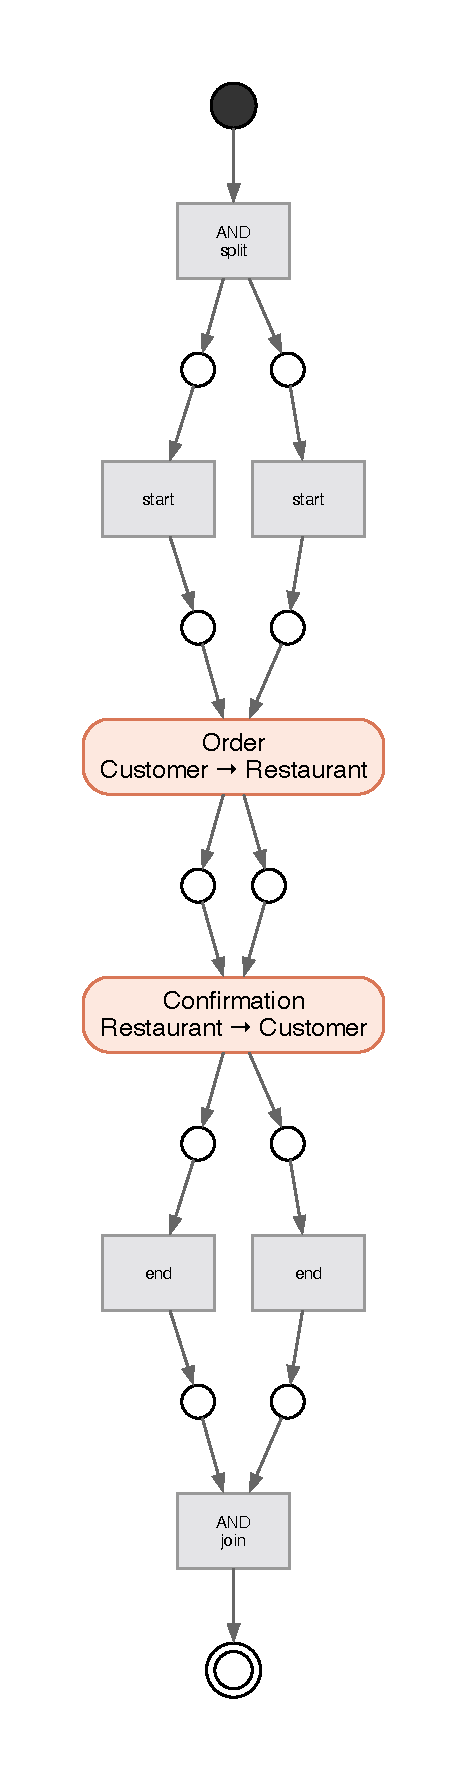
\includegraphics[height=0.5\textheight]{fig-collab-net-tb.pdf}
    \caption{Interaction net generated for the two-pool collaboration-simple
    example. The synthetic AND-split forks the single token into both pools;
    each message exchange is a single transition spanning the two pools; the
    AND-join merges the pools into one end place.}
    \label{fig:collab-net}
\end{figure}

\subsection{Participant and Authorisation Models}
Assigning a single default participant solves the technical need for a caller, but it collapses every task onto one actor. Since access control is often the reason to run a process on a blockchain, we implemented three participant models, selectable through one option and generated from the same diagram: single actor, open, and lane-based.

The \emph{single actor} model is the default described above: one participant is created, and every task is guarded by a check that the caller equals \texttt{participants[0]}. The \emph{open} model drops the caller check entirely, so any account may execute any task the current state allows. This relaxes only authorisation, not ordering: the contract still enforces the sequence of tasks through the token state, but no longer restricts who performs them. The open model therefore suits public processes in which the order matters but the executor does not.

The \emph{lane-based} model derives genuine roles from the diagram. BPMN lanes partition a process by responsibility, and the parser reads the \texttt{laneSet}, \texttt{lane}, and \texttt{flowNodeRef} elements to create one participant per lane and to record which lane owns each task. Each task is then guarded against its own lane's participant. In the example used for the evaluation, the two buyer tasks are checked against \texttt{participants[0]} and the seller task against \texttt{participants[1]}, giving per-role on-chain access control. All three models share the same encoder and backend, and differ only in how participants are assigned during parsing and whether the caller check is emitted during generation. Their on-chain cost is compared in the evaluation.

\subsection{Challenges and Solutions}
The synthetic AND-split and AND-join introduced for collaborations are silent transitions, and like all gateways they name no participant. On a blockchain this raises a question: if no participant owns them, who triggers them? The answer follows from how the generated \texttt{enact} function works. Each call runs a loop that fires every enabled transition whose guard is satisfied, and stops only when it reaches a task that requires an external caller it does not have. Silent transitions carry no guard, so they fire automatically within the first \texttt{enact} call that reaches them, folded into a participant's transaction. They therefore introduce no additional accounts or transactions; the split and join cost only a few units of gas carried by an existing call.

A collaboration file also contains a \texttt{process} element for each pool. Without care, the standalone process translation would run on these inner processes as well and emit a second, incorrect contract for each pool. We guard the process branch so that it runs only when the file contains no collaboration, which ensures that a collaboration is compiled exactly once.

Finally, the event-log reader assumed that every conforming trace contains at least one event. A valid trace can be empty, for instance when a loop's body is skipped, and this caused the reader to fail. A small guard now accepts empty traces, so these cases parse and execute correctly.

% ============================================================================
\section{Quality Assurance and Automated Testing}
\label{sec:testing}

\subsection{Test Suite Architecture}
Chorpiler already includes an automated test suite, organised in three layers, and this work reused it rather than building a new one. The first layer parses every sample model and asserts that a well-formed Interaction Petri Net is produced. The second compiles each net to Solidity and checks that valid contract code is generated. The third and most thorough layer executes the contracts. Each contract is deployed to a local Ethereum Virtual Machine (EVM) provided by Hardhat, and a recorded event log is replayed against it as a sequence of real transactions. A test passes only if every event is accepted in order and the process reaches an empty token state.

Our contribution to this part was not the harness but the test cases that exercise it. The harness discovers its inputs automatically from the model and log directories, so supporting a new diagram type required no new test code: we added a model and a conforming log for each new case, and the existing deploy-and-replay machinery picked them up and ran them. The only change to the harness itself was the small robustness fix to the event-log reader described earlier. That the new diagram types ran through the unchanged pipeline is itself evidence that they are indistinguishable from choreographies at the contract level.

\subsection{Test Data Generation}
For each new diagram type we authored two kinds of test data, both in the XES format: a conforming event log and a non-conforming one. A conforming log is a valid execution that the contract should accept, and the execution layer replays it and checks that the process reaches its end state. A non-conforming log is an invalid execution that the contract should reject, and the same layer replays it and checks that at least one event is refused or that the process never completes. Together with the BPMN model that is deployed, these logs let the suite test both that valid runs succeed and that invalid runs fail.

\subsection{Process Diagram Test Cases}
The process-diagram cases cover the control-flow constructs in isolation. A sequence case checks the basic ordering of tasks. A parallel case exercises an AND-split and AND-join, confirming that both branches must complete before the process continues. An exclusive case exercises an XOR gateway with a default branch and provides one trace for each outgoing branch, so that both the taken and the skipped path are executed. A loop case covers a model that contains a cycle. Each case deploys its contract and replays its conforming log. Each construct is also paired with a non-conforming trace that runs a task before it is enabled. In every case the contract refuses the premature task and the process does not reach its end state.

\subsection{Collaboration Diagram Test Cases}
The collaboration cases focus on message handling across pools. The first uses two pools that exchange two messages in opposite directions, an order from the customer and a confirmation from the restaurant, which tests the merge of a send and a receive task into one transition in both directions. The second adds internal tasks alongside two message flows, checking that internal work and cross-pool communication are handled together within the same collaboration. Both cases deploy to the Hardhat chain and replay their logs successfully. In addition, a non-conforming trace sends the order from the restaurant rather than the customer. The contract rejects it, which confirms that the per-pool access control is enforced on-chain rather than only present in the generated source.

\subsection{Results}
All three layers pass for every model: the parser produces valid nets, the generator produces valid contracts, and all contracts execute their conforming logs to completion on the Hardhat chain, including the new process and collaboration cases. The non-conforming logs are rejected as expected: every invalid ordering is refused, and the order signed by the wrong participant is blocked. The existing choreography tests continue to pass unchanged, which confirms that the extension did not affect the original functionality. 

To compare the three participant models quantitatively, we generated all three from the same lane-annotated process and measured them on the local chain. Table~\ref{tab:gas} reports the deployed bytecode size, the deployment gas, and the gas consumed by the same three-task run.

\begin{table}[t]
\centering
\caption{The three participant models generated from one lane-annotated process
(\texttt{process-lanes.bpmn}), measured on a local EVM.}
\label{tab:gas}
\begin{tabular}{@{}lrrrrl@{}}
\toprule
\textbf{Model} & \textbf{Actors} & \textbf{Code (B)} & \textbf{Deploy gas} &
\textbf{Task gas (total)} & \textbf{Unauth.\ call} \\
\midrule
Open        & 1 & 518 & 215\,636 & 78\,502 & executes \\
SingleActor & 1 & 593 & 231\,806 & 85\,004 & blocked \\
LaneBased   & 2 & 592 & 254\,412 & 85\,004 & blocked \\
\bottomrule
\end{tabular}
\end{table}

The open model is the cheapest in every respect, but it enforces no access control. An unauthorised caller is not rejected, it is simply ignored, because the task's guard is never met. The single-actor and lane-based models cost the same per task, about 2{,}000 gas more than the open model over three tasks, which is the price of the single storage read and comparison that the caller check performs. The lane-based model is no more expensive per task than the single-actor model; it pays only a one-time premium at deployment for storing the second participant address. Per-role access control is therefore essentially free relative to the single-actor approach, while the open model trades all authorisation for its lower cost.

% ============================================================================
\section{Discussion and Evaluation}
\label{sec:discussion}

\subsection{Successes of the Multi-Model Approach}
This work set out to extend Chorpiler from choreographies to two further BPMN diagram types, to provide automated tests for them, and to compare the three types. All three goals were met. Process and collaboration diagrams now compile to smart contracts through the same pipeline as choreographies, and every generated contract was executed on a local blockchain, accepting valid runs and rejecting invalid ones.

The main strength of the approach is that it achieved this by reuse rather than duplication. Because all three diagram types are mapped onto the same Interaction Petri Net, the encoder, the Solidity backend, and the test harness were left almost untouched. A process became a choreography with one participant, and a collaboration became a set of parallel processes joined by message merges. The clearest evidence of this is that the existing test suite validated the new diagram types without any new test code, and that the original choreography tests still pass.

Beyond the assigned scope, the three participant models give process diagrams a range of access-control options. The measurements show that enforcing access control costs about 2{,}000 gas per task, and that deriving roles from lanes is no more expensive per task than using a single actor. Role-based access control is therefore available at essentially no additional running cost, which makes the lane-based model an attractive default for process diagrams that carry role information.

\subsection{Limitations}
Several limitations remain. The most significant concerns loops. A data-based loop is currently encoded so that the loop condition is tested before the loop body, which gives while semantics rather than the do-while semantics that the BPMN model expresses. As a result the body of a loop may be skipped entirely, and the loop test case in the suite only covers the path in which the body is not executed. This behaviour comes from the shared encoding engine rather than from the new front-end code, but it was surfaced by this work and should be addressed.

The collaboration model also makes two simplifying assumptions. First, it treats all pools as starting together and requires all of them to finish, which the synthetic AND-split and AND-join encode directly. Collaborations in which a pool is created conditionally, or in which several instances of a pool run, are therefore not supported. Second, each message flow is matched to a single sender and a single receiver task, so a task cannot act as both the sender of one message and the receiver of another, and message payloads are not yet carried into the generated contract.

Future work should address the loop encoding and extend message handling to cover payloads and tasks that participate in more than one message flow.

% ============================================================================

\section*{Code Access}
The implementation is publicly available in the Chorpiler repository, branch
\texttt{feature/multimodelsupport}:
\url{https://github.com/tomaaam/chorpiler/tree/feature/multimodelsupport}.

% ============================================================================
\begin{thebibliography}{8}

\bibitem{chorpiler}
Stiehle, F.: Chorpiler. GitHub repository.
\url{https://github.com/fstiehle/chorpiler}

\bibitem{dijkman}
Dijkman, R.M., Dumas, M., Ouyang, C.: Semantics and analysis of business process models in BPMN. Information and Software Technology \textbf{50}(12), 1281--1294 (2008)

\bibitem{garcia}
García-Bañuelos, L., Ponomarev, A., Dumas, M., Weber, I.: Optimized execution of business processes on blockchain. In: BPM, pp. 130--146. Springer, Cham (2017)

\bibitem{weber}
Weber, I., Xu, X., Riveret, R., Governatori, G., Ponomarev, A., Mendling, J.:
Untrusted business process monitoring and execution using blockchain. In: BPM
2016. LNCS, vol. 9850, pp. 329--347. Springer, Cham (2016)

\bibitem{bpmnexample}
Object Management Group: Business Process Model and Notation (BPMN) 2.0 by
Example. OMG Document dtc/10-06-02 (2010).
\url{http://www.omg.org/cgi-bin/doc?dtc/10-06-02}

\bibitem{decker}
Decker, G., Weske, M.: Local enforceability in interaction Petri nets. In: BPM 2007. LNCS, vol. 4714, pp. 305--319. Springer, Heidelberg (2007)
\end{thebibliography}

\end{document}